\chapter{Internet of Threads}                %crea il capitolo
%%%%%%%%%%%%%%%%%%%%%%%%%%%%%%%%%%%%%%%%%imposta l'intestazione di pagina
\lhead[\fancyplain{}{\bfseries\thepage}]{\fancyplain{}{\bfseries\rightmark}}
\pagenumbering{arabic}                  %mette i numeri arabi
\section{Definizione}                 %crea la sezione
L'Internet of Things, ovvero l'internet delle cose, vuole rappresentare la diffusione dei sistemi embedded come veri e propri nodi di reti. Nell'ottica dell'IoT, oggi, apparecchi comuni in un'abitazione, quali condizionatore, la caldaia o addirittura il tostapane, possono essere nodi di rete ed essere quindi configurati e controllati attraverso di essa.\\
Il concetto di Internet of Threads \`e una evoluzione di questa astrazione. L'idea alla base di IoTh \`e quella di avere non solo oggetti ma anche processi come nodi di rete.\\
Per poter capire pienamente i vantaggi dell'IoTh si pu\`o pensare ad un'analogia con quanto \`e successo nel mondo della telefonia. In passato la telefonia collegava apparecchi fissi connessi via cavo. In questo modello il numero di telefono individuava un luogo e non una persona e quindi era comune, per trovare una persona, doversi interrogare sul dove questa potesse essere; al contrario l'avvento dei telefoni cellulari ha cambiato l'idea di significato di numero di telefono, non pi\`u associato a luoghi fisici ma ad una persona infatti i telefoni cellulari sono normalmente telefoni personali\cite{K1,K2}.\\
Come possiamo notare infatti, con questa tecnologia lo stack \`e direttamente integrato nel programma.
\begin{figure}[h]
     \begin{center}%
        \subfigure[stack associato all'interfaccia fisica]{%
            \label{fig:physical}
            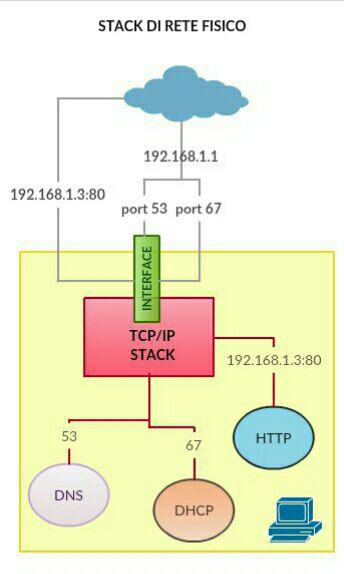
\includegraphics[width=7cm]{old_stack}
        }%
        \subfigure[stack associato ai processi]{%
           \label{fig:virtual}
           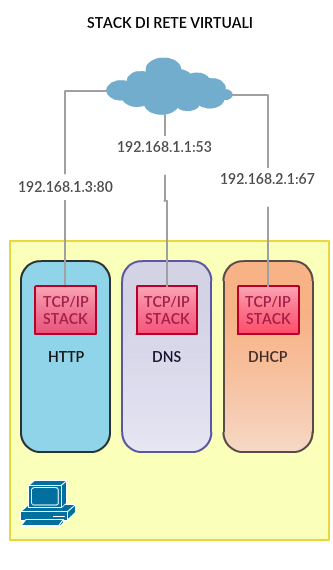
\includegraphics[width=7cm]{new_stack}
        }
%
    \end{center}
    \caption{%
        Differenze tra stack reali e virtuali
     }%
\end{figure}%\
Nello stesso modo IoTh indirizza i processi che forniscono un servizio, significa che questi processi non sono pi\`u vincolati a risiedere in un luogo specifico, o in un elaboratore specifico nell'ambito delle reti, ma \`e possibile trasparentemente farli migrare da un elaboratore all'altro senza che questo crei difficolt\`a di indirizzamento.\\
Una nota va anche fatta in termini di sicurezza. La possibilit\`a che ogni servizio utilizzi propri indirizzi IP e uno stack di rete privato rende molto pi\`u difficile se non praticamente impossibile sfruttare le fragilit\`a di un servizio per poter scalare l'intrusione ad altri servizi presenti su di esso.

\section{Stack Implementati}
Diversi sono i progetti che si occupano di offrire ai processi il proprio stack di rete; tra questi ne verranno presi in esame tre, considerati pi\`u indicati per uno studio in quanto open source. Ognuno di essi offre la propria implementazione di stack di rete.\\
Uno stack di rete legato al processo permette di connettere lo stesso ad una rete reale, tramite le interfacce fornite dal sistema, o virtuale (ad esempio VDE) come se fosse una macchina fisica a se stante, a questo punto ogni processo pu\`o staccarsi dal modo in cui la macchina che lo ospita gestisce la rete ed avere le proprie regole.\\

\subsection{PicoTCP}
PicoTCP\cite{K4} \`e supportato da Tass Belgium (Altran); \`e lo stack pi\`u conosciuto e diffuso per sistemi embedded ed esistono anche dei progetti basati su IP di reti mesh realizzati con picoTCP\cite{K14}.\\
PicoTCP presenta una struttura modulare (schema molto utilizzato per questo tipo di progetto come vedremo in seguito), che permette di avere il minimo indispensabile all'interno dell'applicazione.\\
Vanta la compatibilit\`a con un gran numero di dispositivi costruiti con diversi processori e interfacce di rete, pu\`o essere compilato con diversi compilatori ed \`e gi\`a integrato in alcuni sistemi nati per ridurre al minimo il consumo di risorse.\\
Purtroppo a causa di incompatibilit\`a con la licenza GPL alcune parti del codice non sono state rese pubbliche anche se rappresentano una piccola percentuale dell'intero progetto.
\subsection{LWIP}
Nasce come progetto di Adam Dunkels pensato per sistemi embedded ma che inizialmente non forniva supporto ad IPv6.\\
Light-weight IP (LWIP\cite{K13}) vanta un core molto piccolo e la possibilit\`a di eseguire anche senza sistema oprativo (single-threaded) e con il minor consumo di RAM possibile, inoltre \`e modulare ed offre la possibilit\`a di aggiungere protocolli come DHCP e DNS solo in caso di necessit\`a.\\
Supporta sia little che big endian e gira su processori a 8 e 32 bit, quindi funziona anche su un semplice ATMEGA.\\
Unica pecca \`e il protoccolo IPv6 che \`e ancora in fase sperimentale, infatti il supporto IPv6 pu\`o essere aggiunto ed \`e scaricabile da git.
\subsection{LWIPv6}
LWIPv6 nasce per colmare la mancanza del supporto IPv6 in LWIP, ed \`e questo uno dei motivi della nascita di LWIPv6\cite{K6}.\\
\begin{description}                     %crea un elenco descrittivo
  \item[virtualsquare\cite{K15}: ] un progetto ideato da Renzo Davoli e Michael Goldweber. Comprende una gamma di tool pensati per sperimentare e creare strumenti di uso comune in tema di virtualizzazione.
\end{description}
Quando al team di virtualsquare \`e sopravvenuta la necessit\`a di avere uno stack per la rete vde non esisteva ancora nulla di maturo o comunque plug and play, da questa esigenza il team ha pensato di realizzare uno stack versatile in versione libreria tale per cui ogni processo potesse avere il proprio stack di rete.\\
Caratteristica principale di LWIPv6 \`e il suo motore ibrido che, di fatto funziona solo con IPv6 e mappa in questo protocollo le comunicazioni IPv4.\\
La conversione degli indirizzi ip da IPv4 ad IPv6 \`e particolare ma intuitiva. I 32 bit finali dell'indirizzo IPv6 rappresentano quello in versione 4, i 16 bit antecedenti sono settati a 1 e la parte restante, i primi 80 bit, a 0. Di seguito un esmpio sull'indirizzo 192.168.1.2:
\begin{table}[h]                        %ambiente tabella
                                        %(serve per avere la legenda)
\begin{center}                          %centra nella pagina la tabella
\begin{tabular}{r|c|c|c}                  %tre colonne con righe verticali
                                        %   prodotte con |
\hline
$IP version$ & $80 bit$ & $16 bit$ & $32 bit$\\
\hline \hline                         %inserisce due righe orizzontali
$IPv4$ & $unused$  & $unused$  & $192.168.1.2$\\           %& separa le colonne e con
\hline                                  %inserisce una riga orizzontale
$IPv6$ & $00000000.00000000.0000$ & $FFFF$ & $192.168.1.2$\\           %  \\ va a capo
\hline                                  %inserisce una riga orizzontale
$IPv6$ & $00000000.00000000.0000$ & $FFFF$ & $C0A80102$\\
\hline                           %inserisce due righe orizzontali
\end{tabular}
\caption[IPv4 to IPv6 conversion]{rappresentazione di un indirizzo IPv4 in IPv6}\label{tab:IPv4toIPv6}
\end{center}
\end{table}

Per quanto riguarda le maschere per\`o questa configurazione non pu\`o essere adottata. Se i primi 80 bit venissero settati a 0 non sarebbero considerati e nel caso in cui due reti differissero proprio nei primi 80 bit non potremmo pi\`u smistare i pacchetti verso la corretta rete di destinazione.\\
LWIPv6 si caratterizza perch\'e tramite una modifica della conversione non ha bisogno di usare due motori diversi per IPv4 ed IPv6 ma uno che \`e ibrido. La modifica \`e semplice ed \`e stato sufficiente ribaltare i primi 80 bit. Come prima suggeriamo un esempio di conversione di una maschera all'interno di LWIPv6:

\begin{table}[h]                        %ambiente tabella
                                        %(serve per avere la legenda)
\begin{center}                          %centra nella pagina la tabella
\begin{tabular}{r|c|c|c}                  %tre colonne con righe verticali
                                        %   prodotte con |
\hline
$IP version$ & $80 bit$ & $16 bit$ & $32 bit$\\
\hline  \hline        %inserisce due righe orizzontali
$IPv4$ & $unused$  &  $unused$  & $255.255.255.0$\\           %& separa le colonne e con
\hline                                  %inserisce una riga orizzontale
$IPv6$ & $FFFFFFFF.FFFFFFFF.FFFF$ & $FFFF$ & $255.255.255.0$\\           %  \\ va a capo
\hline                                  %inserisce una riga orizzontale
$IPv6$ & $FFFFFFFF.FFFFFFFF.FFFF$ & $FFFF$ & $FFFFFF00$\\
\hline                           %inserisce due righe orizzontali
\end{tabular}
\caption[IPv4 to IPv6 mask conversion]{rappresentazione delle maschere in LWIPv6}\label{tab:IPv4toIPv6 mask}
\end{center}
\end{table}
\section{Netlink}
\subsection{Inter Process Communication(IPC)}
Molti processi necessitano di scambiare informazioni per i motivi pi\`u disparati, dalla comunicazione di rete a quella interna ad una sola macchina.\\
\`E banalmente limitativo pensare di costruire solo programmi fini a se stessi e che quindi non comprendano nessuna interazione con altri programmi.\\
Con IPC intendiamo quindi l'insieme delle tecnologie adottate per permettere ai processi di comunicare tra essi, che siano ospitati sulla stessa macchina o distribuiti sulla rete, tra queste tecnologie esiste appunto quella utilizzata all'interno della libreria VsnLib di cui parleremo nello specifico del prossimo capitolo..
\subsection{Il Sistema IPC Netlink}
Netlink \`e un sistema IPC adottato dal kernel linux perch\'e in grado di mettere in comunicazione diversi task, solitamente serve per far comunicare task in user-space con task in kernel-space ma pu\`o far interagire anche processi entrambi in user-space.\\
Studiato per essere il successore di ioctl per le configurazioni ed il monitoraggio, si propone di essere pi\`u flessibile.
Ma come avviene esattamente la comunicazione attraverso netlink?\\
Netlink utilizza un sistema di socket indicizzato in base ai processi ogni processo pu\`o definire socket diversi di tipo netlink (AF\_NETLINK, NETLINK\_GENERIC, NETLINK\_XFRM) per inviare e ricevere messaggi con e da altri processi, implementa un sistema di porte basato sul process ID dei processi; ad esempio per la comunicazione con il kernel viene usata la porta 0.\\
L'immagine successiva rende perfettamente il concetto.
\begin{figure}[h]                       %crea l'ambiente figura; [h] sta
                                        %   per here, cio� la figura va qui
\begin{center}                          %centra nel mezzo della pagina
                                        %   la figura
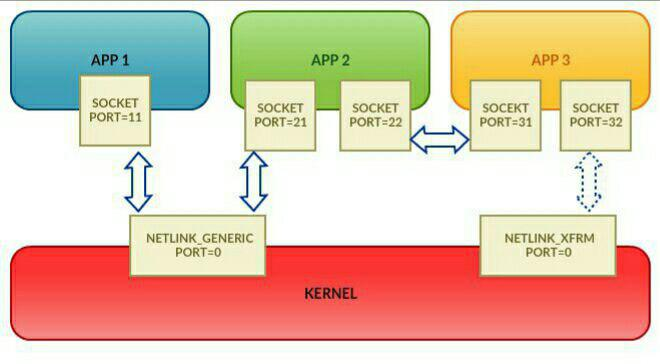
\includegraphics[width=10cm]{netlink_comunication}%inserisce una figura larga 5cm
                                        %se si vuole usare va scommentata
%
%%%%%%%%%%%%%%%%%%%%%%%%%%%%%%%%%%%%%%%%%inserisce la legenda ed etichetta
                                        %   la figura con \label{fig:prima}
\caption[comunicazione netlink]{scambio di messaggi attraverso socket netlink}
\end{center}
\end{figure}\\
L'interfaccia di comunicazione \`e abbastanza standardizzata ma il payload \`e personalizzabile ed \`e possibile definire la propria struttura da utilizzare per inviare dati (informazioni), tra processi diversi, attraverso i socket netlink.
\begin{figure}[h]                       %crea l'ambiente figura; [h] sta
                                        %   per here, cio� la figura va qui
\begin{center}                          %centra nel mezzo della pagina
                                        %   la figura
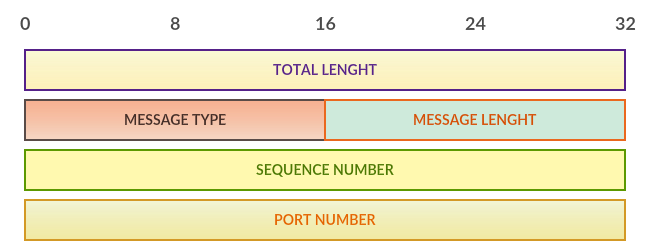
\includegraphics[width=8cm]{nlmsghdr}%inserisce una figura larga 5cm
                                        %se si vuole usare va scommentata
%
%%%%%%%%%%%%%%%%%%%%%%%%%%%%%%%%%%%%%%%%%inserisce la legenda ed etichetta
                                        %   la figura con \label{fig:prima}
\caption[struct nlmsghdr]{schema della struttura nlmsghdr}
\end{center}
\end{figure}\\
\subsection{Libnl}
Netlink Protocol Library Suite (libnl) \cite{K10}, \`e una raccolta di librerie ed utility che forniscono API di comunicazione netlink basate su quelle del kernel linux e comprende:
\begin{description}                     %crea un elenco descrittivo
  \item[libnl] Core della libreria, offre uno strato di unificazione delle interfacce sulle quali poi si basano le altre librerie che pertanto di pendo da questa;
  \item[libnl-route] Questa libreria si occupa di fornire API per la configurazione degli elemnti della famiglia NETLINK\_ROUTE;
  \item[libnl-genl] genl significa generic netlink e questa libreria offre una versione estesa del protocollo netlink;
  \item[libnl-nf] API per configurazioni netlink basate su netfilter.

\end{description}
%%%%%%%%%%%%%%%%%%%%%%%%%%%%%%%%%%%%%%%%%non numera l'ultima pagina sinistra

\clearpage{\pagestyle{empty}\cleardoublepage}
